% Title: Text Generation with Python
% Author: Matt Rogers
% Written for the Boston Python NLP study group
% Presented on 18 Aug 2022

% Beamer configuration
\documentclass[10pt,aspectratio=169]{beamer}

% Input encoding
\usepackage[utf8]{inputenc}

% graphicx package
\usepackage{graphicx}
\graphicspath{{figures/}}

% tcolorbox package
\usepackage{tcolorbox}

% TikZ package
\usepackage{tikz}

% hyperref package
\usepackage{hyperref}
\hypersetup{colorlinks=true}

% Presentation info
\author{Matt Rogers}
\title{Text Generation with Python}
\date{18 August 2022} 

% Presentation content
\begin{document}

\section{Title Page}
\begin{frame}
\titlepage
\end{frame}


\section{Session Aims}
\begin{frame}
\frametitle{Session Aims}
\begin{columns}

	\begin{column}{0.6\textwidth}
		In this session, we will...
		
		\vspace{12pt}
		
		\begin{itemize}
		\item Introduce natural language generation (NLG)\\
		      from a system-building perspective
		
		\item Provide an overview of the design process\\
		      of an NLG system
		
		\item Design and implement a simple NLG system\\
		      in Python using real data
		\end{itemize}
	\end{column}
	
	\begin{column}{0.4\textwidth}
		\centering
		
\includegraphics[width=0.8\textwidth]{pexels-saliha-7871270}
	\end{column}

\end{columns}
\end{frame}


\section{Overview of NLG}
\begin{frame}
\frametitle{Overview of NLG}

\begin{quote}
	Natural language generation (NLG) ... is concerned with the
	construction of computer systems that can produce understandable texts
	in English or other human languages from some underlying
	non-linguistic representation of information.
	
	\vspace{6pt}
	
	\footnotesize E. Reiter and R. Dale. ``Building applied natural
	language generation systems.'' (1997)
\end{quote}

\vspace{12pt}

Some common applications of NLG:

\vspace{12pt}

\begin{columns}

	\begin{column}{0.5\textwidth}
	\begin{itemize}
	
	\item Provide analysis and interpretation of business data
		
	\item Generate textual weather forecasts from data and maps
	
	\item Explain medical information to patients
	
	\end{itemize}
	\end{column}
	
	\begin{column}{0.5\textwidth}
	\begin{itemize}
	
	\item Automate customer service communications
	
	\item Caption images
	
	\item Write computational humor
	
	\end{itemize}
	\end{column}

\end{columns}

\end{frame}


\section{Requirements Analysis}
\begin{frame}
\frametitle{Requirements Analysis}

\begin{columns}

	\begin{column}{0.65\textwidth}
		The first step in building a system is \textbf{requirements analysis}:
		Determining user expectations for what the system does.
		
		\vspace{12pt}
		
		For an NLG project, this	involves assembling a collection
		of input and output data called a \textbf{corpus}.
		
		\vspace{12pt}
		
		Example: A system that takes railway timetable data as input,
		and produces a textual description that users (passengers) can understand.
		
	\end{column}
	
	\begin{column}{0.35\textwidth}
		\begin{center}
		% Illustration of data -> text for requirements analysis

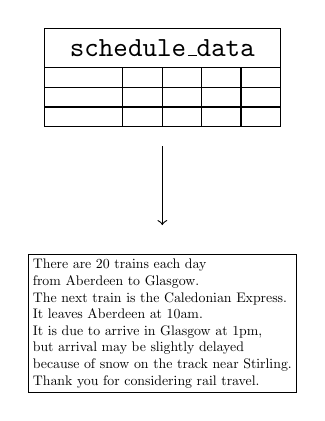
\begin{tikzpicture}

\draw (0, 1.00) -- (3, 1.00);
\draw (0, 1.25) -- (3, 1.25);
\draw (0, 1.50) -- (3, 1.50);
\draw (0, 1.75) -- (3, 1.75);
\draw (0, 2.25) -- (3, 2.25);

\draw (0.0, 1.00) -- (0.0, 2.25);
\draw (1.0, 1.00) -- (1.0, 1.75);
\draw (1.5, 1.00) -- (1.5, 1.75);
\draw (2.0, 1.00) -- (2.0, 1.75);
\draw (2.5, 1.00) -- (2.5, 1.75);
\draw (3.0, 1.00) -- (3.0, 2.25);

\node at (1.5, 2) {\texttt{schedule\_data}};

\draw [->] (1.5, 0.75) -- (1.5, -0.25);

\node [rectangle, draw, align=left, scale=0.5] at (1.5, -1.5) {
	There are 20 trains each day\\
	from Aberdeen to Glasgow.\\
	The next train is the Caledonian Express.\\
	It leaves Aberdeen at 10am.\\
	It is due to arrive in Glasgow at 1pm,\\
	but arrival may be slightly delayed\\
	because of snow on the track near Stirling.\\
	Thank you for considering rail travel.
};

\end{tikzpicture}
		\end{center}
	\end{column}

\end{columns}

\end{frame}
\begin{frame}
\frametitle{Requirements Analysis (cont'd)}

We need to analyze the information content of the corpus text.

Classify each sentence or clause into one of the following categories:

\vspace{12pt}

\begin{center}
\begin{tabular}{|l|l|}
\hline
\textbf{Category} & \textbf{Example} \\
\hline
Unchanging text & Thank you for considering rail travel. \\
\hline
Directly-available data & The next train is the Caledonian Express. \\
\hline
Computable data & There are 20 trains each day \\
 & from Aberdeen to Glasgow. \\
\hline
Unavailable data & There is snow on the track near Stirling. \\
\hline
\end{tabular}
\end{center}

\vspace{12pt}

By classifying sentences into categories, we get a better sense
of the difficulty and cost of implementing different requirements.
In the case of unavailable data, implementing the requirement
may be prohibitively expensive or impossible.

\end{frame}


\section{NLG Tasks}
\begin{frame}
\frametitle{NLG Tasks}

\begin{columns}
	
	\begin{column}{0.6\textwidth}
		Big picture: Transform input data to output text...\\
		But what are the actual processes involved?

		\vspace{12pt}
		
		\begin{itemize}
		
			\item \textbf{Content determination} \\
			      Decide what information to convey\\
			      Identify \textit{entities}, \textit{concepts},
			      and \textit{relations}\\
			      Create data objects called \textit{messages}
		
			\item \textbf{Discourse planning} \\
			      Impose ordering and structure over the messages
			
			\item \textbf{Sentence aggregation} \\
			      Group messages together into sentences
		
		\end{itemize}
	\end{column}
	
	\begin{column}{0.4\textwidth}
	\tiny
		\begin{tcolorbox}[title=message-id: msg01, width=0.85\textwidth]
			relation: IDENTITY
			
			arg1: NEXT-TRAIN
			
			arg2: CALEDONIAN-EXPRESS
		\end{tcolorbox}
		
		``The next train is the Caledonian Express.''
		
		\vspace{12pt}
		
		\begin{tcolorbox}[title=message-id: msg02, width=0.85\textwidth]
			relation: DEPARTURE
			
			departing-entity: CALEDONIAN-EXPRESS
			
			departure-location: ABERDEEN
			
			departure-time: 1000
		\end{tcolorbox}
		
		``The Caledonian Express leaves Aberdeen at 10am.''
	\end{column}

\end{columns}

\end{frame}

\begin{frame}
\frametitle{NLG Tasks (cont'd)}

\begin{columns}

	\begin{column}{0.4\textwidth}
		\centering
		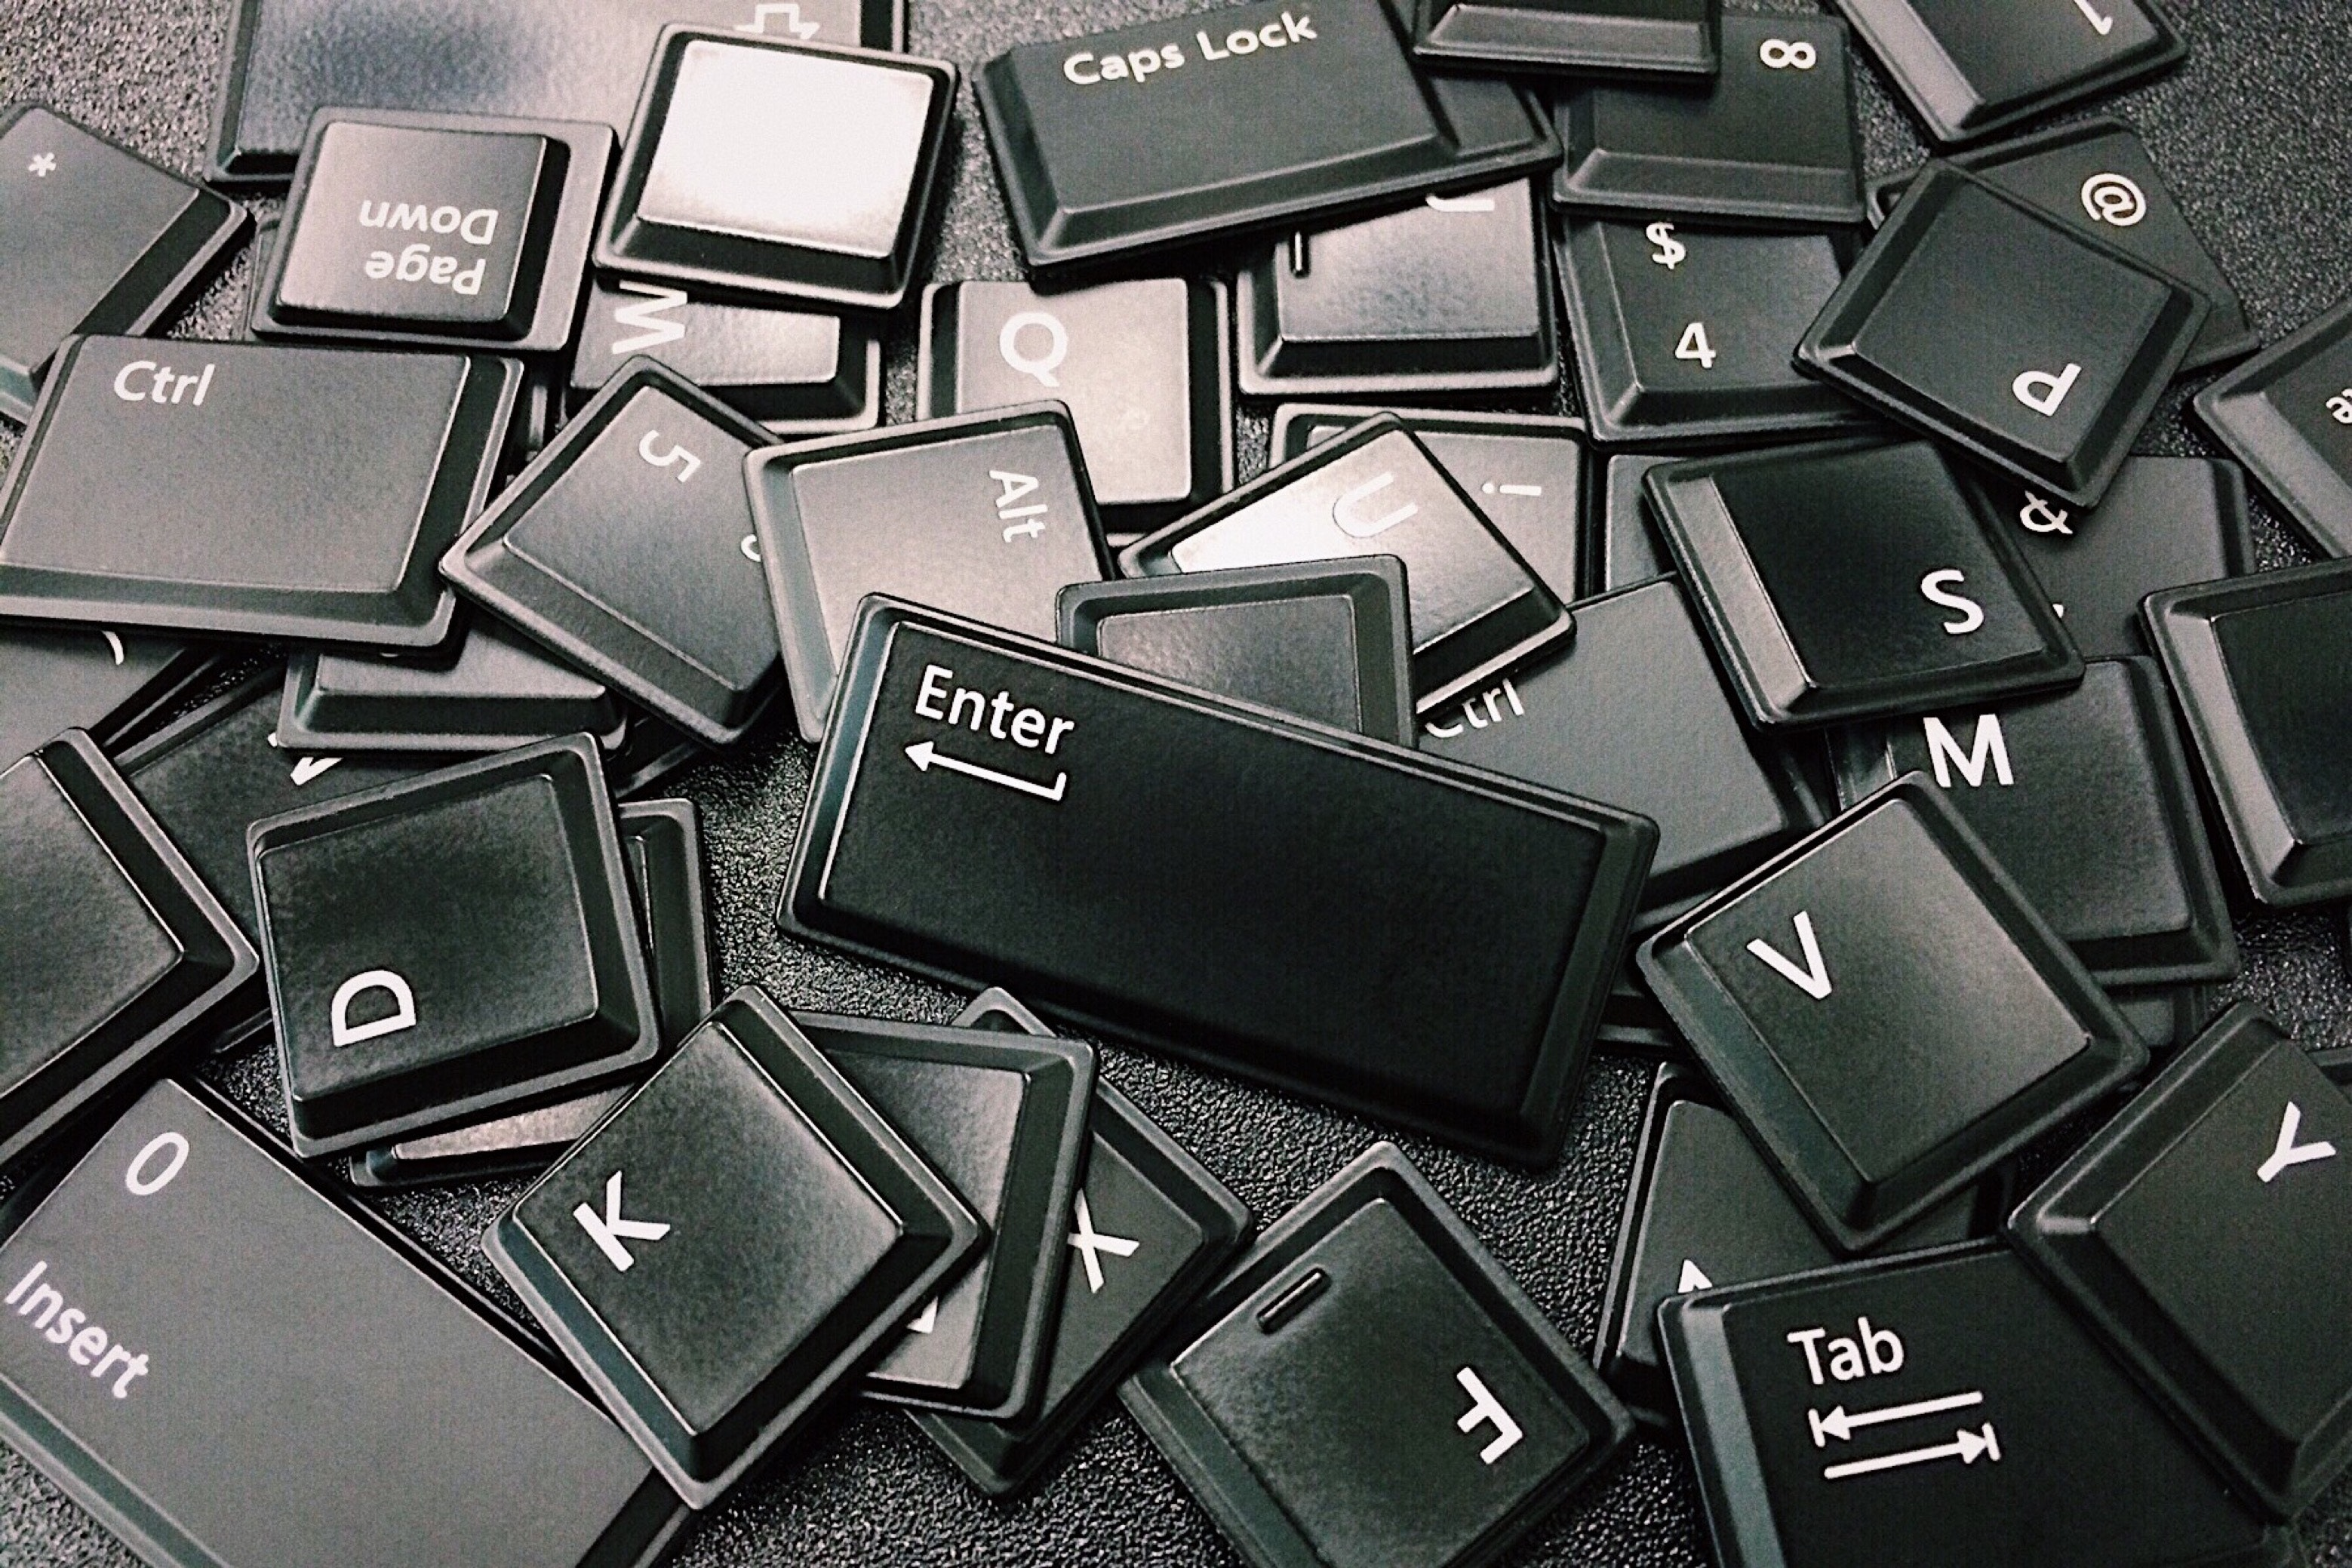
\includegraphics[angle=90,width=0.8\textwidth]{pexels-pixabay-373072}
	\end{column}
	
	\begin{column}{0.6\textwidth}
	
		\begin{itemize}
		
			\item \textbf{Lexicalization} \\
			      Choose specific words and phrases
			      to convey the concepts and relations
			      appearing in the messages
			      
			\item \textbf{Referring expression generation} \\
			      Select words or phrases to identify domain entities
			
			\item \textbf{Linguistic realisation} \\
			      Apply the rules of grammar to produce text
		
		\end{itemize}
		
		\vspace{12pt}
		
		A given task may be very complex in some systems,\\
		and very simple in others.
		
		\vspace{12pt}
		
		It depends on the requirements!
	
	\end{column}

\end{columns}

\end{frame}


\section{NLG System Architecture}
\begin{frame}
\frametitle{NLG System Architecture}

Reiter and Dale suggest a three-stage pipeline:

\vspace{12pt}

\begin{center}
% Illustration of three-stage NLG system architecture
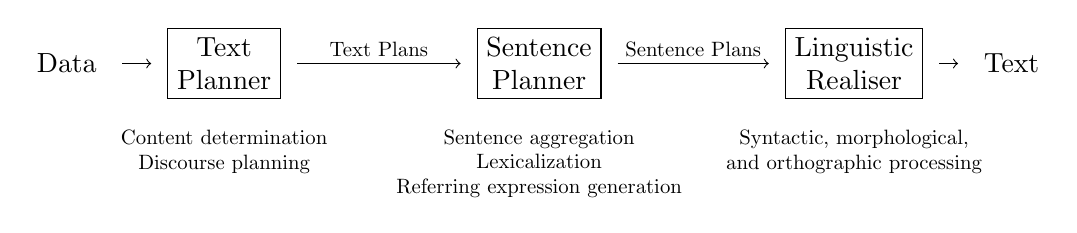
\begin{tikzpicture}

\node(0) [align=center, outer sep=6pt] at (-2, 0) {Data};

\node(1) [rectangle, draw, align=center, outer sep=6pt] at (0, 0) {Text \\ Planner};
\node [align=center, scale=0.75, below of=1, anchor=north] {
	Content determination\\
	Discourse planning
};

\node(2) [rectangle, draw, align=center, outer sep=6pt] at (4, 0) {Sentence \\ Planner};
\node [align=center, scale=0.75, below of=2, anchor=north] {
	Sentence aggregation\\
	Lexicalization\\
	Referring expression generation
};

\node(3) [rectangle, draw, align=center, outer sep=6pt] at (8, 0) {Linguistic \\ Realiser};
\node [align=center, scale=0.75, below of=3, anchor=north] {
	Syntactic, morphological,\\
	and orthographic processing
};

\node(4) [align=center, outer sep=6pt] at (10, 0) {Text};

\draw [->] (0) -- (1);
\draw [->] (1) to node[above, scale=0.75] {Text Plans} (2);
\draw [->] (2) to node[above, scale=0.75] {Sentence Plans} (3);
\draw [->] (3) -- (4);

\end{tikzpicture}

\end{center}

\vspace{12pt}

We need two more data objects to represent the data passed between
stages in the pipeline:

\begin{itemize}
	\item \textbf{Text plans} specify messages and how they are conceptually grouped
	\item \textbf{Sentence plans} specify templates or abstract representations of sentences
\end{itemize}
\end{frame}


\section{NLG Project: Weather Report}
\begin{frame}
\frametitle{Mini-Project: Generating a Weather Report}

\begin{columns}

	\begin{column}{0.6\textwidth}
		The National Weather Service makes available an API
		providing critical forecasts, alerts, observations,
		and other weather data products.
		
		\vspace{12pt}
		
		Let's design and implement an NLG system
		that takes local forecast data as input,
		and produces a textual report
		of the most relevant features in the forecast.
	\end{column}
	
	\begin{column}{0.4\textwidth}
		\centering
		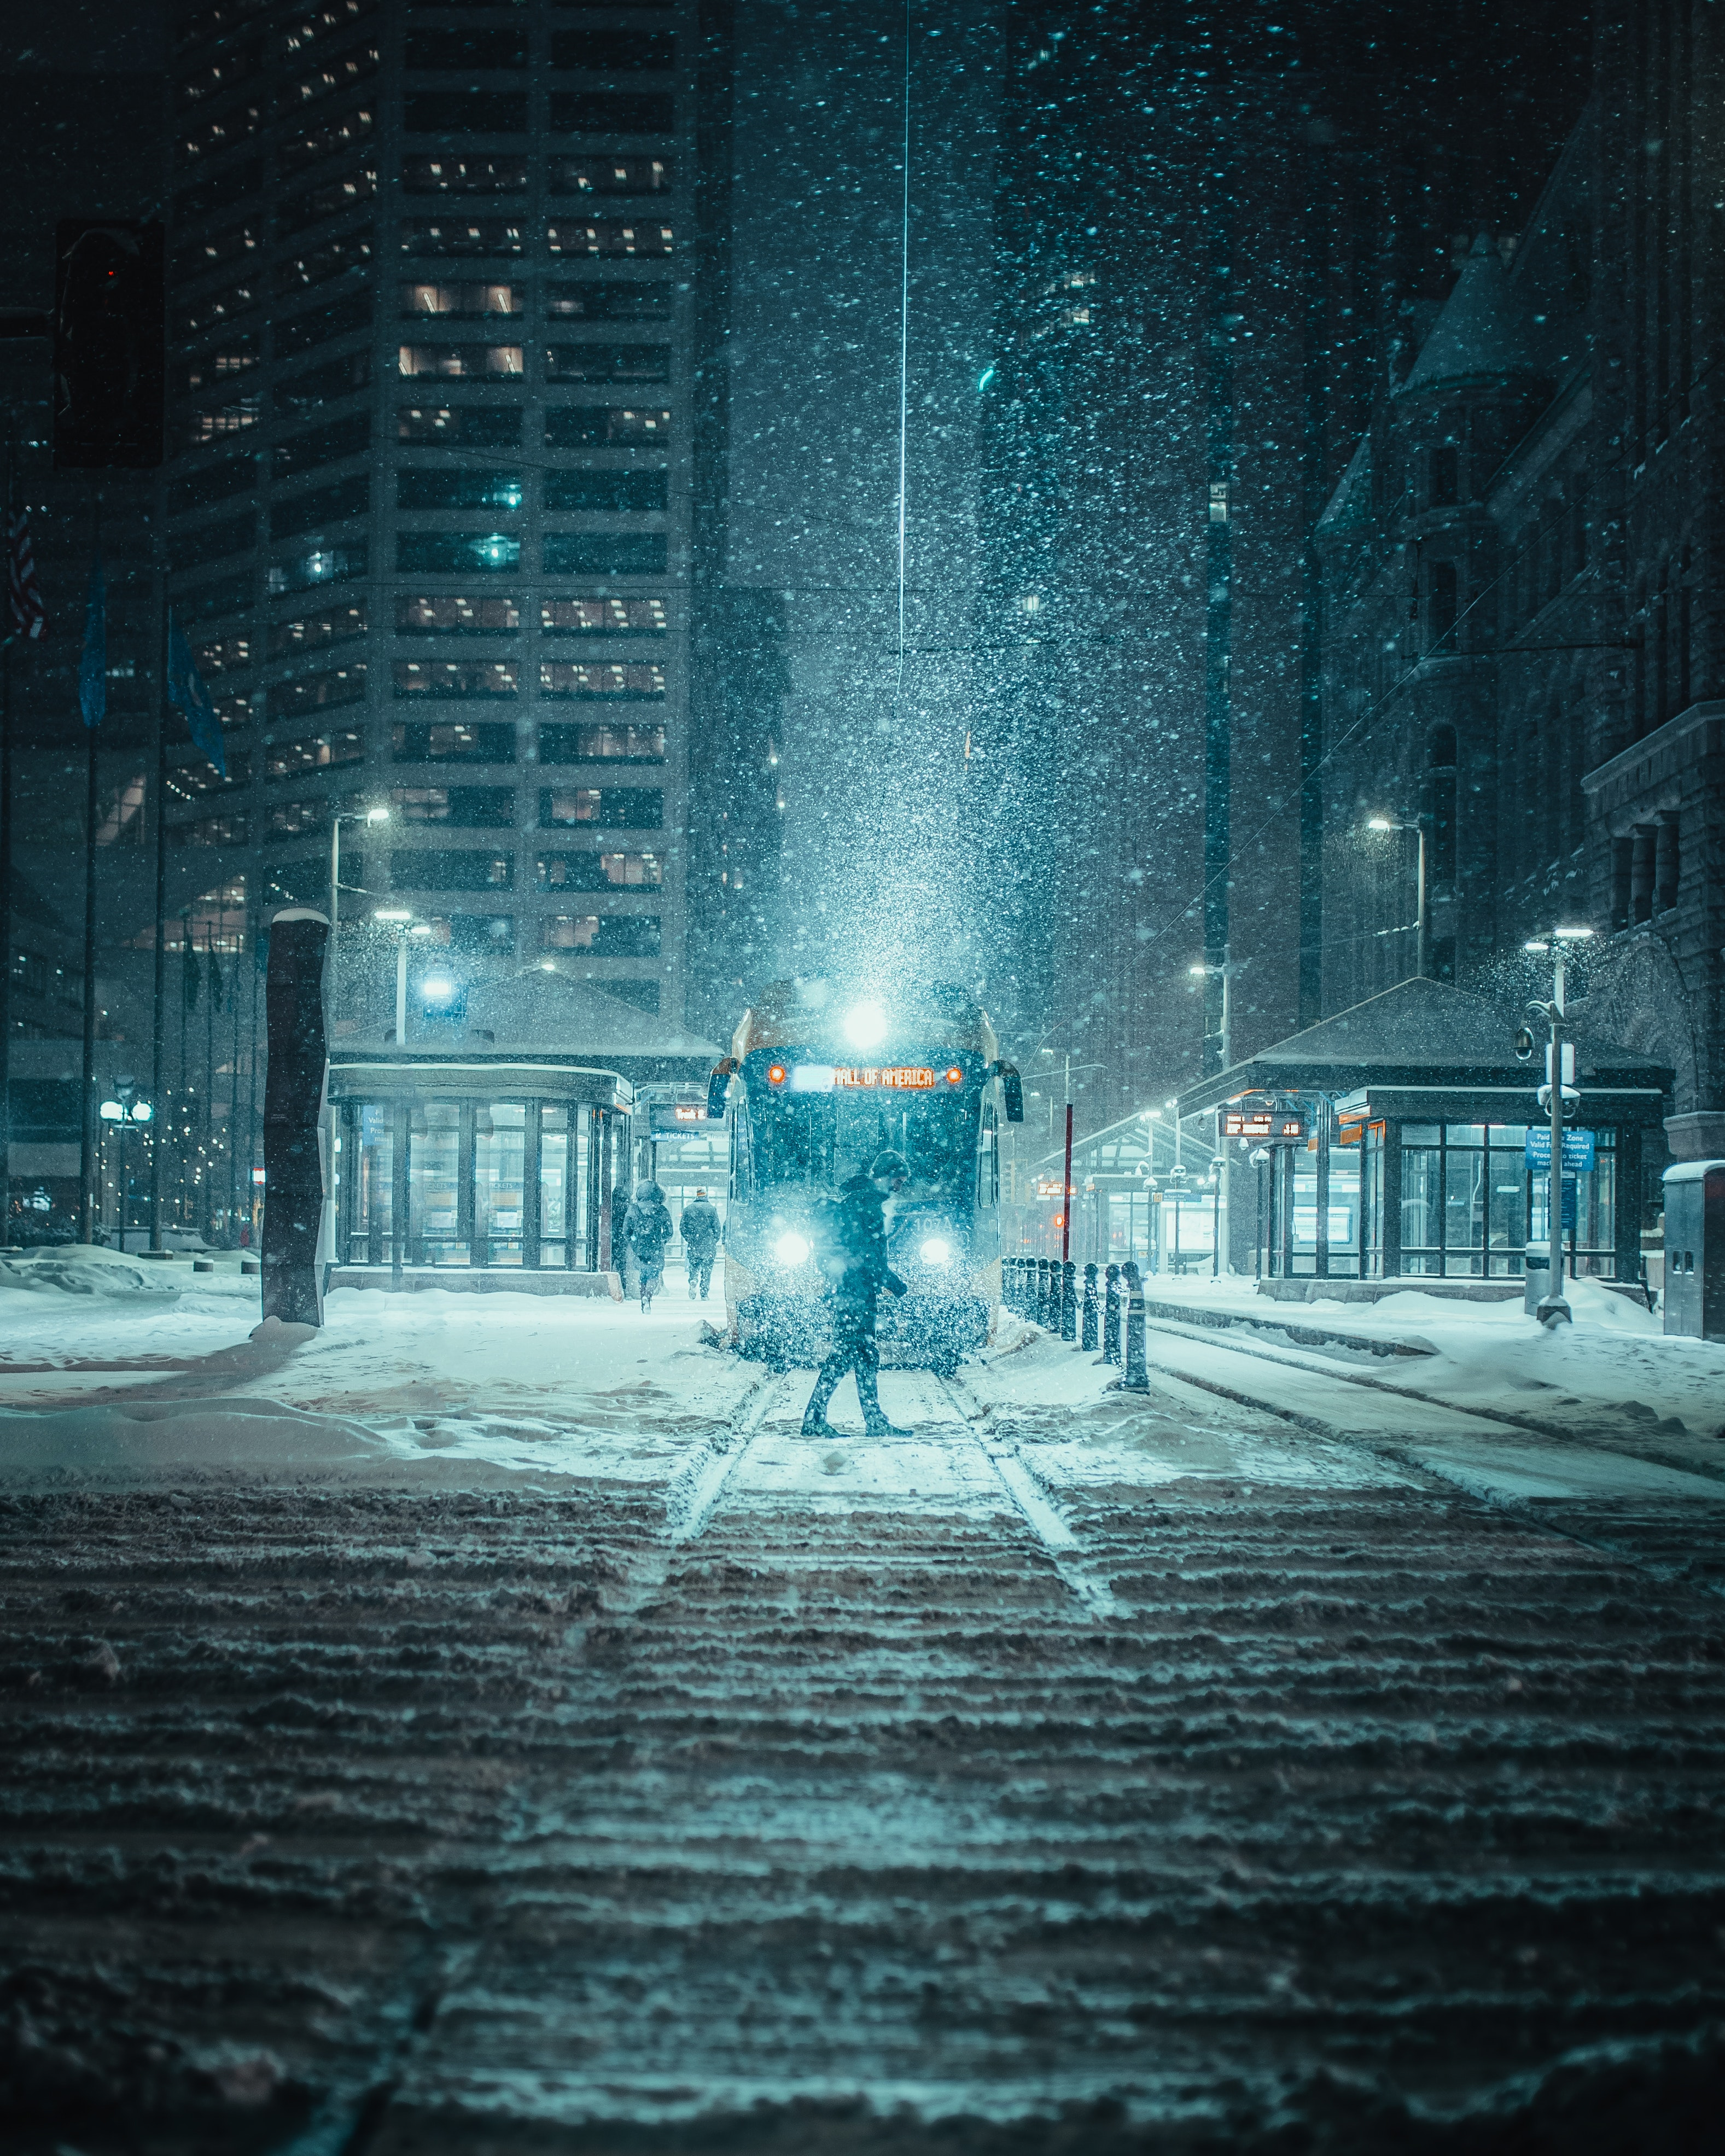
\includegraphics[width=0.8\textwidth]{pexels-josh-hild-2422497}
	\end{column}

\end{columns}

\vspace{12pt}

Documentation: \href{https://www.weather.gov/documentation/services-web-api}{https://www.weather.gov/documentation/services-web-api}

API: \href{https://api.weather.gov/}{https://api.weather.gov/}


\end{frame}
\begin{frame}
\frametitle{Mini-Project: Requirements Analysis}

First, consider system use cases and constraints.

\vspace{24pt}

\begin{columns}

	\begin{column}{0.5\textwidth}
		Use Cases
		
		\begin{itemize}
			
			\item As a traveler, I want to read a brief overview
			of the forecast at my destination.
			
			\item As an event planner, I want to include
			the forecast in a welcome email to attendees.
			
			\item As a community organizer, I want to post
			the forecast to a bulletin board.
			
		\end{itemize}
		
	\end{column}
	
	\begin{column}{0.5\textwidth}
		Constraints
		
		\begin{itemize}
		
			\item The NWS API has reasonable rate limits
			to prevent abuse of the system.
			
			\item Data covers no more than 7 days ahead.
			
			\item Forecast features are limited to temperature, wind speed
			and direction, cloud cover, and precipitation.
		
		\end{itemize}
		
	\end{column}

\end{columns}

\end{frame}
\begin{frame}
\frametitle{Mini-Project: Requirements Analysis (cont'd)}

Assemble a \textbf{corpus} consisting of input data and output text.

\vspace{12pt}

\begin{center}

\texttt{\scriptsize
\begin{tabular}{|l|l|l|l|l|l|}
\hline
id & name            & startTime & temp & wind & forecast \\
\hline
1  & This Afternoon  & 2022-08-14T16:00:00  & 82  & 6 mph        & Partly Sunny \\
2  & Tonight         & 2022-08-14T18:00:00  & 61  & 2 to 6 mph   & Mostly Cloudy \\
3  & Monday          & 2022-08-15T06:00:00  & 81  & 2 to 7 mph   & Mostly Sunny \\
4  & Monday Night    & 2022-08-15T18:00:00  & 62  & 2 to 6 mph   & Mostly Cloudy \\
5  & Tuesday         & 2022-08-16T06:00:00  & 77  & 5 to 13 mph  & Mostly Sunny \\
6  & Tuesday Night   & 2022-08-16T18:00:00  & 63  & 6 to 10 mph  & Slight Chance Rain Showers \\
7  & Wednesday       & 2022-08-17T06:00:00  & 73  & 9 to 14 mph  & Rain Showers Likely \\
8  & Wednesday Night & 2022-08-17T18:00:00  & 62  & 7 to 10 mph  & Chance Rain Showers \\
 & & & \vdots & & \\
\hline
\end{tabular}
}

\vspace{12pt}

$\downarrow$

\vspace{12pt}

\texttt{
Temperatures will range from the 60s to the 80s.\\
Rain is predicted for Tuesday night through Wednesday night.\\
Winds above 12 mph are predicted for Tuesday and Wednesday.
}

\end{center}

\end{frame}
\begin{frame}
\frametitle{Mini-Project: Requirements Analysis (cont'd)}

Classify each of the sentences we want to generate.

\vspace{12pt}

\begin{center}
	\begin{tabular}{|l|l|}
		\hline
		\textbf{Sentence} & \textbf{Category} \\
		\hline
		Temperatures will range from &  Directly-available data \\
		the 60s to the 80s.  & \\
		\hline
		Rain is predicted for Tuesday night  & Computable data \\
		through Wednesday night.  & \\
		\hline
		Winds above 12 mph are predicted  & Computable data \\
		for Tuesday and Wednesday.  & \\
		\hline
	\end{tabular}
\end{center}

\vspace{12pt}

The temperature range is directly available by selecting the minimum
and maximum temperature values from the source table.

\vspace{12pt}

Periods of rain and high wind are not directly available, but are computable.

We need to identify when periods of interest begin and end.

\end{frame}
\begin{frame}
\frametitle{Mini-Project: Text Planning}

What relations are we expressing?

\begin{itemize}
	\item A value (\textit{temperature}) will vary within a range.
	\item A weather condition (\textit{rain}, \textit{winds above 12 mph})
	will occur during a period of time.
\end{itemize}

\vspace{12pt}

What kinds of messages can we use to express these relations?

\vspace{12pt}

\begin{tcolorbox}[width=0.45\textwidth,nobeforeafter,title=Message]
	relation: VALUE-IN-RANGE
	
	value: TEMPERATURE
	
	minimum: 61
	
	maximum: 82
\end{tcolorbox}
\hfill
\begin{tcolorbox}[width=0.45\textwidth,nobeforeafter,title=Message]
	relation: CONDITION-IN-PERIOD
	
	condition: RAIN
	
	period-start: TUESDAY-NIGHT
	
	period-end: WEDNESDAY-NIGHT
\end{tcolorbox}


\end{frame}
\begin{frame}
\frametitle{Mini-Project: Text Planning (cont'd)}

The typical output of the text planner will be:

\begin{itemize}
	\item One message about temperature.
	
	\item Zero, one, or several messages about weather conditions.
	
	\item Several messages may refer to the same condition (e.g. rain)
	at different time periods (e.g. Tuesday-Wednesday and Friday-Saturday).
\end{itemize}

\vspace{12pt}

Discourse planning: The temperature information is produced first.

\vspace{12pt}

Information about weather conditions should be grouped by condition.\\
The groups should be produced in the order that the conditions first occur.

\vspace{12pt}

For example, if today is Thursday, then we should
talk about the rain that's expected Friday before we talk about the
high winds predicted for Sunday.

\end{frame}
\begin{frame}
\frametitle{Mini-Project: Sentence Planning}

The sentence planner takes the structured messages and produces a sentence plan.

How it accomplishes this task depends on the relation in the messages:

\vspace{12pt}

\textbf{Relation: value-in-range}

The text plan consists of a single message.

\vspace{12pt}

\begin{center}
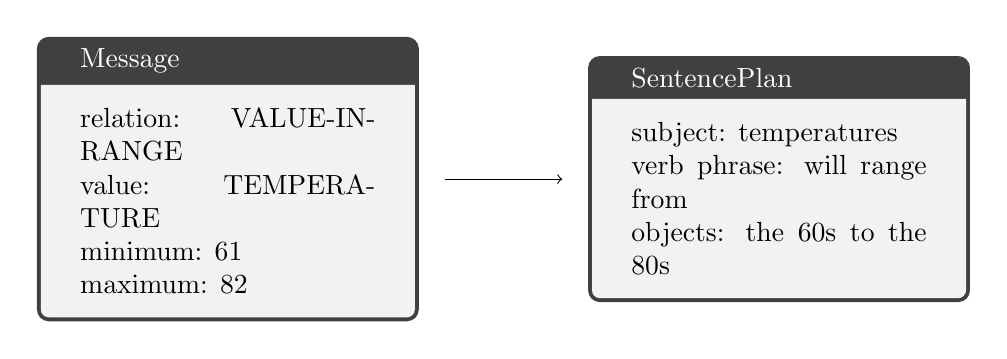
\begin{tikzpicture}
\node (1) [outer sep=6pt] at (0,0) {
\begin{tcolorbox}[width=0.4\textwidth,nobeforeafter,title=Message]
relation: VALUE-IN-RANGE

value: TEMPERATURE

minimum: 61

maximum: 82
\end{tcolorbox}
};

\node (2) [outer sep=6pt] at (7,0) {
\begin{tcolorbox}[width=0.4\textwidth,nobeforeafter,title=SentencePlan]
subject: temperatures

verb phrase: will range from

objects: the 60s to the 80s
\end{tcolorbox}
};

\draw [->] (1) -- (2);

\end{tikzpicture}
\end{center}

\end{frame}
\begin{frame}
\frametitle{Mini-Project: Sentence Planning (cont'd)}


\textbf{Relation: condition-in-period}

The text plan consists of one or more messages to aggregate
into one sentence.

\vspace{12pt}

\begin{center}
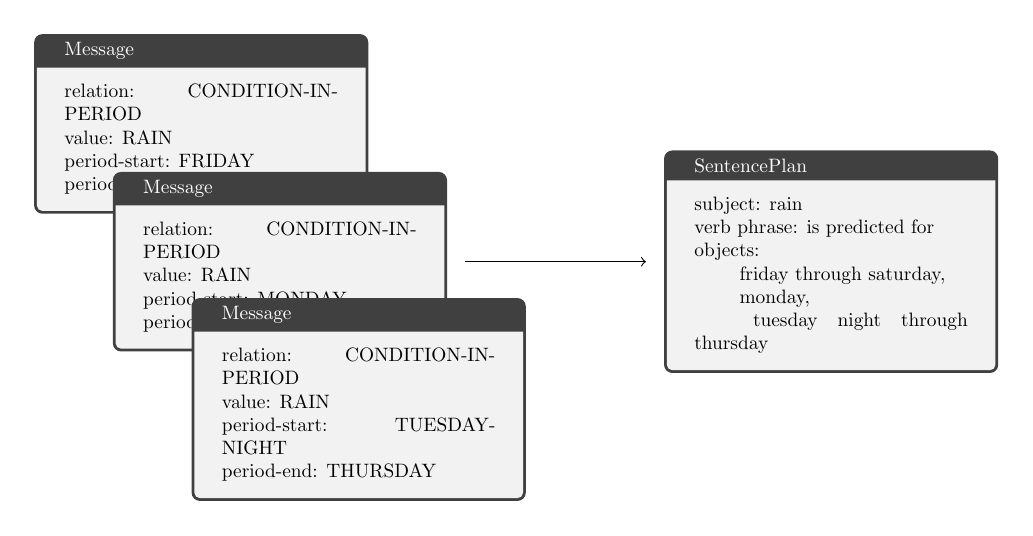
\begin{tikzpicture}

\node (0) [scale=0.7, outer sep=6pt] at (-1,1.75) {
\begin{tcolorbox}[width=0.5\textwidth,nobeforeafter,title=Message]
relation: CONDITION-IN-PERIOD

value: RAIN

period-start: FRIDAY

period-end: SATURDAY
\end{tcolorbox}
};

\node (1) [scale=0.7, outer sep=6pt] at (0,0) {
\begin{tcolorbox}[width=0.5\textwidth,nobeforeafter,title=Message]
relation: CONDITION-IN-PERIOD

value: RAIN

period-start: MONDAY

period-end: MONDAY
\end{tcolorbox}
};

\node (2) [scale=0.7, outer sep=6pt] at (1,-1.75) {
\begin{tcolorbox}[width=0.5\textwidth,nobeforeafter,title=Message]
relation: CONDITION-IN-PERIOD

value: RAIN

period-start: TUESDAY-NIGHT

period-end: THURSDAY
\end{tcolorbox}
};

\node (3) [scale=0.7, outer sep=6pt] at (7,0) {
\begin{tcolorbox}[width=0.5\textwidth,nobeforeafter,title=SentencePlan]
subject: rain

verb phrase: is predicted for

objects: 

\hspace{2em} friday through saturday,

\hspace{2em} monday,

\hspace{2em} tuesday night through thursday
\end{tcolorbox}
};

\draw [->] (1) -- (3);

\end{tikzpicture}
\end{center}

\end{frame}
\begin{frame}
\frametitle{Mini-Project: Linguistic Realisation}

The linguistic realiser puts the sentence together according to the rules of grammar.

\vspace{12pt}

We plug the data from the sentence plan into a template,
add conjunctions and punctuation, adjust pluralization if needed,
and adjust capitalization:

\vspace{12pt}

\begin{center}
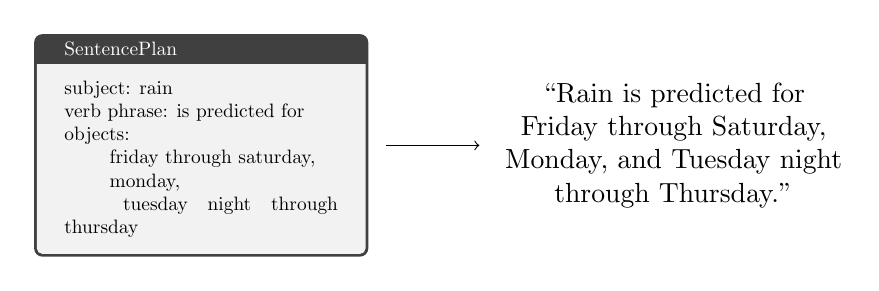
\begin{tikzpicture}

\node (1) [scale=0.7, outer sep=6pt] at (0,0) {
\begin{tcolorbox}[width=0.5\textwidth,nobeforeafter,title=SentencePlan]
subject: rain

verb phrase: is predicted for

objects: 

\hspace{2em} friday through saturday,

\hspace{2em} monday,

\hspace{2em} tuesday night through thursday
\end{tcolorbox}
};

\node (2) [align=center, outer sep=6pt] at (6,0) {
``Rain is predicted for \\ Friday through Saturday, \\
Monday, and Tuesday night \\ through Thursday.''
};

\draw [->] (1) -- (2);

\end{tikzpicture}
\end{center}

\end{frame}
\begin{frame}
\frametitle{Mini-Project: Architecture}

\begin{center}
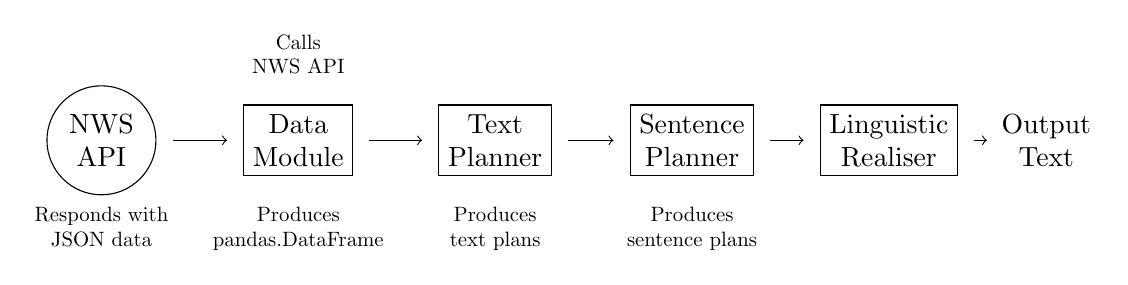
\begin{tikzpicture}

\node (1) [draw, circle, align=center, outer sep=6pt] at (0, 0) {NWS \\ API};
\node [align=center, scale=0.75, below of=1, anchor=north] {Responds with \\ JSON data};

\node (2) [draw, rectangle, align=center, outer sep=6pt] at (2.5, 0) {Data \\ Module};
\node [align=center, scale=0.75, above of=2, anchor=south] {Calls \\ NWS API};
\node [align=center, scale=0.75, below of=2, anchor=north] {Produces \\ pandas.DataFrame};

\node (3) [draw, rectangle, align=center, outer sep=6pt] at (5, 0) {Text \\ Planner};
\node [align=center, scale=0.75, below of=3, anchor=north] {Produces \\ text plans};

\node (4) [draw, rectangle, align=center, outer sep=6pt] at (7.5, 0) {Sentence \\ Planner};
\node [align=center, scale=0.75, below of=4, anchor=north] {Produces \\ sentence plans};

\node (5) [draw, rectangle, align=center, outer sep=6pt] at (10, 0) {Linguistic \\ Realiser};
\node [align=center, scale=0.75, below of=5, anchor=north] {};

\node (6) [align=center, outer sep=2pt] at (12, 0) {Output \\ Text};

\draw [->] (1) -- (2);
\draw [->] (2) -- (3);
\draw [->] (3) -- (4);
\draw [->] (4) -- (5);
\draw [->] (5) -- (6);

\end{tikzpicture}
\end{center}

\vspace{12pt}

The \textbf{NWS API} is a web resource that produces the data of interest.

\vspace{12pt}

The \textbf{data module} contains methods to retrieve data from the API,
and defines the data objects used in the NLG pipeline:
\textit{Message}, \textit{TextPlan}, and \textit{SentencePlan}.

\vspace{12pt}

The \textbf{text planner}, \textbf{sentence planner},
and \textbf{linguistic realiser} modules form the NLG pipeline.

\end{frame}
\begin{frame}
\frametitle{Mini-Project: Implementation and Live Demo}

\begin{center}
Now let's walk through the code and see it in action!
\end{center}

\end{frame}

\section{Thanks}
\begin{frame}
\frametitle{Thank You!}

Many thanks to the organizers and members of the Boston Python User Group\\
for making this session possible.

\vspace{24pt}

The presentation and project code are available on my GitHub:

\href{https://github.com/mrogers-ebsco/bospy-textgen}{https://github.com/mrogers-ebsco/bospy-textgen}
\end{frame}

\end{document}